\documentclass{protokol}
\leftheader{Objevování částic v detektoru ATLAS v CERN}
\centerheader{}
\rightheader{Tomáš Derner}

\begin{document}

  \section*{Úkol}

    \begin{enumerate}
      \item Zpracujte přibližně 50 událostí z detektoru ATLAS programem Hypatia
      \item Pomocí programu ROOT zobrazte histogram invariantních hmotností pro různě velké statistické soubory
      \item Identifikujte výrazné píky a přiřaďte je očekávaným částicím
      \item Zjistěte chybu střední hodnoty invariantní hmotnosti pro nalezené částice pro různě velké statistické soubory
      \item Vyneste zjištěné chyby do grafu jako funkci počtu událostí a srovnejte je s Poissonovým rozdělením 
    \end{enumerate}

  \section*{Teorie}

    Elementární částice důležité pro toto praktikum jsou Z boson, Higgsův boson a J$/\psi$ a $\Upsilon$ mesony. Z boson zprostředkovává elektroslabou interakci, má hmotnost $\SI{91}{GeV/c\squared}$. Higgsův boson je poslední objevená částice Standardního modelu, má hmotnost $\SI{125}{GeV/c\squared}$. Hmotnosti částic J$/\psi$ a $\Upsilon$ jsou $\SI{3.01}{GeV/c\squared}$, resp. $\SI{9.46}{GeV/c\squared}$.

    Tyto částice mají krátkou dobu života, detekují se tedy jen jejich rozpadové produkty. Podle druhu těchto částic a jejich energií můžeme zpětně určit identitu původní částice. Je proto dobré energii rozpadových částic přepočítat na invariantní hmotnost \cite{pokyny}
    \begin{equation}
      m_0 = \sqrt{ \left( \frac{ E }{ c^2 } \right)^2 - \left( \frac{ \vec{p} }{ c } \right)^2 }.
    \end{equation}
    
    Tuto hmotnost můžeme srovnat s hmotností původní částice.

    Při zpracování událostí můžeme najít rozpady na dvě nebo čtyři částice: $e^+ e^-$, $\mu^+ \mu^-$, $\gamma \gamma$, $e^+ e^- e^+ e^-$, $\mu^+ \mu^- \mu^+ \mu^-$ a $ e^+ e^- \mu^+ \mu^-$.

  \section*{Výsledky}

    Pomocí programu Hypatia bylo zpracováno 100 událostí ze tří souborů. 

    \subsection*{Úkol 2 a 3}

      Pomocí makra dostupného v praktiku byly v programu ROOT zobrazeny histogramy invariantních hmotností částic určených v úkolu 1. Příloha 1 níže obsahuje histogramy pro částici Z, příloha 3 histogramy pro Higgsův boson. První tři grafy v obou přílohách ukazují invariantní hmotnosti všech zpracovaných událostí v různém přiblížení. 
      
      Oblasti hodnot invariantní hmotnosti odpovídající předpokládaným částicím byly fitovány gaussovou křivkou. Je zřejmé, že zatímco fity polohy částice Z byly úspěšné, fit histogramu s největším přiblížením pro Higgsův boson dává nesmyslné výsledky. To lze vysvětlit tím, že ve 100 událostech se Higgsův boson nevyskytuje dostatečně krát na to, aby byl jeho odpovídající pík v histogramu dobře definován.

      Následujících 6 histogramů v příloze 1 a 3 zobrazují pouze události označené jako určitý typ interakce, viz teorie. Ačkoliv tyto histogramy v obou přílohách zobrazují tu samou informaci, z důvodu různého výchozího nastavení rozpětí horizontální osy a velikosti binu vypadají značně odlišně. Výchozí nastavení těchto histogramů byla ponechána z důvodu naší nedostatečné znalosti programu ROOT.

      V příloze 2 a 4 jsou zobrazeny výsledky zpracování 3814 událostí. Zatímco je tento počet událostí dostatečný k pohodlné identifikaci píku částice Z, pík odpovídající Higgsově bosonu není zřetelný.

      Příloha 5 obsahuje histogramy pro meson $\Upsilon$ a J$/\psi$, které jsou význačné výrazně menší invariantní hmotností než Z a Higgs. Histogramy jsou vytvořeny z 3814 událostí, pouhých 100 nestačilo na vytvoření definovaných píků.

    \subsection*{Úkol 4 a 5}

      Jediná částice, jejíž pík je dobře definovaný už při 100 událostech je Z částice. Proto používáme tento pík pro určení chyby $\sigma$ střední hodnoty invariantní hmotnosti pro soubory 100, 200, 500 a 3814 událostí. Použité histogramy jsou zobrazeny v příloze 6, závislost chyby na počtu událostí zaznamenaná v tabulce \ref{tab:u4} a v grafu \ref{fig:u5}. Závislost v grafu \ref{fig:u5} nepřipomíná Poissonovo rozdělení.

      \begin{table}[H]
        \centering
        \setlength{\tabcolsep}{10pt}
        \begin{tabular}[t]{
  S[table-format=4.0]
  S[table-format=1.3]
  S[table-format=1.3]
} \toprule
{Počet událostí} & {Chyba střední hodnoty $\sigma$} & {Chyba chyby} \\ \midrule
             100 &                            4.963 &         0.848 \\
             200 &                            3.266 &         0.344 \\
             500 &                            3.389 &         0.310 \\
            3814 &                            3.885 &         0.123 \\ \bottomrule
\end{tabular}
        \caption{Tabulka chyb určení střední hodnoty invariantní hmotnosti pro různě velké soubory událostí}
        \label{tab:u4}
      \end{table}

      \begin{figure}[H]
        \centering
        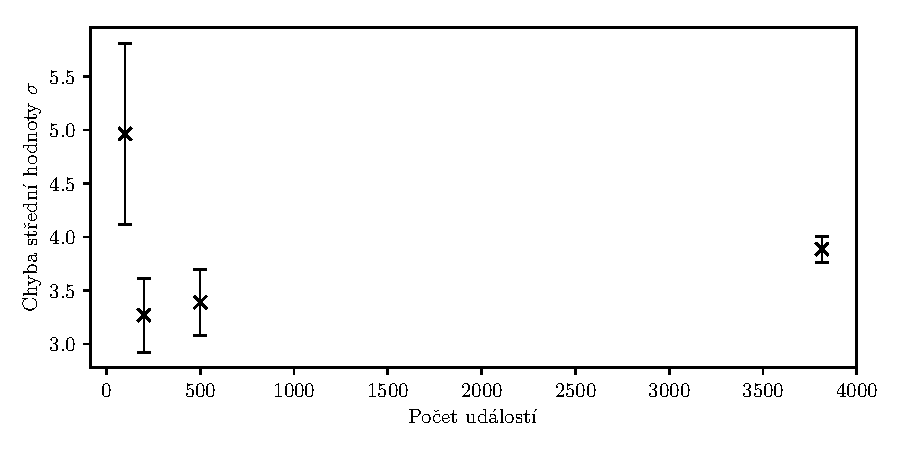
\includegraphics[]{u5}
        \vspace{-15pt} 
        \caption{Graf závislosti chyb určení střední hodnoty invariantní hmotnosti na počtu událostí}
        \label{fig:u5}
      \end{figure}

  \section*{Diskuse}

    Vzhledem k povaze úlohy byla veškerá diskuse provedena v sekci výsledků.


  \section*{Závěr}

    Programem Hypatia bylo zpracováno 100 událostí, z těchto byly vytvořeny histogramy invariantních hmotností. Tytéž histogramy byly vytvořeny z 3814 předchozích zpracování.

    Zjištěné chyby středních hodnot invariantní hmotnosti neodpovídají Poissonovu rozdělení.


  \begin{thebibliography}{}
 
    \bibitem{pokyny}
    Pokyny k měření ``Objevování částic v detektoru ATLAS v
    CERN'', dostupné z\\ \url{https://physics.mff.cuni.cz/vyuka/zfp/_media/zadani/texty/txt_401.pdf}, 22.\,10.\,2018
   
  \end{thebibliography}

\end{document} 